\chapter{A model of Group-based Emotions}
\label{chapter:group-based-emotions}

% RESEARCH QUESTION can the expression of group-based emotions by a robotic teammate increase people's identification and trust with the team?

The current chapter describes to our approach towards the third research goal -- \textit{develop computational mechanisms for the robotic teammate to improve collective cohesion}. One of the motivations behind this particular part of our work is the fact that the autonomous robotic agents (previously mentioned in Chapters~\ref{chapter:membership-formation} and \ref{chapter:pro-sociality}) were developed on top of an architecture for emotional agents. According to the group identity theory, there is a particular group of emotions that reflects a high level of identification with the group, which are called the group-based emotions. This idea led us to formulate the following research question: can the expression of group-based emotions by a robotic teammate increase people's identification and trust towards the team?

The current chapter starts with a brief background on group-based emotions in Section~\ref{sec:backgroup}. Then, we propose an implementation for the group identification process in Section~\ref{sec:model} and, in Section~\ref{sec:model-implementation}, we provide a detailed description of how it was applied in our card game scenario. The chapter proceeds with a user study to evaluate the model in Section~\ref{sec:study4} and a detailed discussion of the results in Section~\ref{sec:study4-discussion}. Section~\ref{sec:concluding-remarks} concludes with some considerations and remarks.


\section{Background}
\label{sec:backgroup}
Group-based emotions are believed to be a result of self-ca\-te\-go\-ri\-sa\-tion and appraisal theories of emotions \cite{smith1993social}. When the social identity of the perceiver leads him to think of himself as a \textit{group member} rather than just an individual, events affecting his in-group may elicit such type of group emotions. Naturally, these emotional reactions occur during intergroup interaction and, according to Smith \cite{smith1993social}, the salience of social identity is elicited by 3 factors: (1) the presence of out-group members, (2) the perception of similarities with the in-group members, and (3) the competition between groups. A quite common example of a group-based emotion is the feeling of pride or shame for our favourite sports team.


Recently, Goldenberg et al. have proposed a process model of group-based emotions  \cite{goldenberg2016process} that extends the ``modal model'' of Gross \& Thompson \cite{Gross2007}. The extension of a general model of emotion to account for group-based emotions is supported by the notion that these emotions, although different in their appraisals, have the same basic structure as regular emotions. 

In this model, the process of generating group-based emotions, starts with an attention allocation to a given situation or stimuli. Then, the relevance of the situation being attended is conditioned by the group identity that the individual associates himself at the moment and how strong is that association. Finally, the process ends with an emotional response that may range from the expression of emotions to organised actions.

During intergroup interactions, there is a close relation between group-based emotions and group identification. Group identification was known as being an antecedent of group-based emotions until Kessler and Hollbach \cite{kessler2005group} have presented how group-based emotions can influence group identification and, therefore, how they can have bidirectional causality. Their results point to the fact that in-group identification may increase or decrease according to the type of emotions and the target being the in-group or the out-group. In particular, happiness towards the in-group and anger towards the out-group increase in-group identification, the same way happiness towards the out-group and anger towards the in-group decrease in-group identification. The authors also reveal a positive correlation between the intensity of emotions increasing identification and the final identification level, which may lead to a positive feedback loop that explains the development of a collective action frame.

\section{A model of group-based emotions for social robotic characters}
\label{sec:model}

Social robotic characters can generate group-based emotions in similar contexts as humans if they are equipped with mechanisms that properly approximate the human psychological process that leads to these emotions. Our model (see Figure \ref{fig:model}) is aimed in this direction with its mechanisms being grounded on the recent psychological model of group-based emotions, proposed by Goldenberg et al. \cite{goldenberg2016process}.

\begin{figure}[ht]
\centering
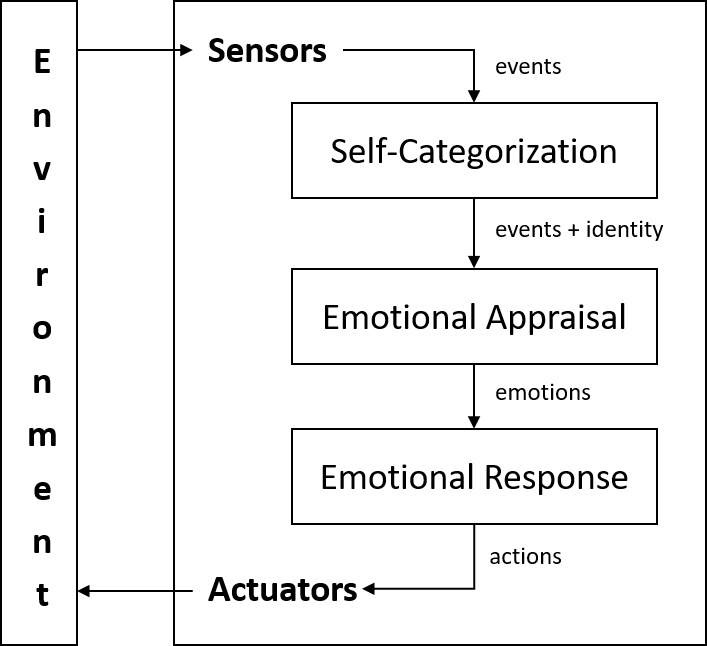
\includegraphics[width=0.3\textwidth]{images/gbe/model.png}
\caption{Diagram of the group-based emotions model.}
\label{fig:model}
\end{figure}


The first component of the model is the \textit{Self-Categorisation} component, which is responsible for managing the current context of the interaction as well as the social groups that are present in that context, if any, and their members. These elements constitute a social layer on top of the physical reality that is being perceived by the robot's sensors. Based on the Self-Categorisation Theory \cite{hornsey2008social,turner1987rediscovering}, when the robot detects a presence of an out-group then its own group identity will become more salient. 

The emotional appraisal is the second component of the model. This component is responsible for generating emotions in response to the events that occur within the current social context. An event can correspond to a performance of an action or to a change in a property of the environment. For each event perceived, the emotional component performs a series of value judgements about that event in relation to the robot. Then, a set of emotions are synthesised in accordance to those judgements. In emotional psychology, these judgements are referred to as appraisal variables with different theories of emotion proposing different sets of variables \cite{moors2013appraisal}. For instance, according to the OCC theory \cite{ortony1990cognitive}, when someone judges an event to be desirable for him or her, that person is likely to experience joy afterwards in proportion to the level of desirability attributed. The same theory also proposes that when someone performs an action that is considered blameworthy than that person is inclined to feel shame. However, if the blameworthy action is performed by another person, then a reproach emotion is felt instead by the observer.

While many researchers have already been able to integrate an emotional appraisal component in a social robotic architecture, the innovative aspect of our model lies in the notion that our appraisal component is capable of considering a social group as the actor of an event even if, in reality, all actions are being performed by individuals. This is the result of introducing the \textit{Self-Categorisation} component before the appraisal takes place in order to determine whether the robot sees itself and others acting based on their individual or their group identity. In the latter case, actions performed by individuals that are sharing the same group identity in the current context are appraised as if they are actions performed by the robot itself. Consequently, in a context where the robot is performing a team-based activity and one of its partners performs a blameworthy action, the appraisal component will generate in the robot a group-based emotion of shame, rather than a reproach emotion towards its partner.

Finally, the last component of the model is the \textit{Emotional Response} component, which is responsible for managing how the robot expresses the emotions that result from the appraisal process. This process must take into account the different possibilities that are afforded by the robot's embodiment. Assuming the robot has the ability to change its facial expression and body posture then these are matched to the current emotional state of the robot. In addition to non-verbal signals, the dialogue acts chosen by the robot are also influenced by its emotions. This is particularly important when trying to convey social emotions such as admiration or pride that can be hard to distinguish from more basic emotions as the ones proposed by Ekman \cite{ekman1987universals}, using only non-verbal modalities.

\begin{algorithm}[ht]
\caption{Group-based emotions generation process}
\label{algorithm-loop}
\begin{algorithmic}
\WHILE {\emph{true}}
\STATE$self \leftarrow Robot.Name $
\STATE$e \leftarrow Sensors.PerceiveNewEvent() $
\STATE$SG \leftarrow ContextManager.GetSalientSocialGroups() $ 
\IF{$SG \neq \emptyset $} 
\STATE$g \leftarrow IdentityManager.SelfCategorisation(SG, self)$ 
\IF{$e.ResponsibleAgent \in g$} 
\STATE $e.ResponsibleAgent \leftarrow g.Name$
\STATE $self \leftarrow g.Name$
\ENDIF
\ENDIF
\STATE$AV \leftarrow Appraisal.DetermineVariables(e)$
\STATE$E \leftarrow Appraisal.GenerateEmotions(AV, self)$
\STATE$se \leftarrow StrongestEmotion(E)$
\FORALL{$c \in Actuators.GetEmotionChannels()$}
\STATE$Express(se, c)$
\ENDFOR
\ENDWHILE
\end{algorithmic}
\end{algorithm}

Algorithm~\ref{algorithm-loop} provides a more detailed view of how these three components work together in a continuous cycle to create group-based emotions. As shown, the cycle starts by defining the parameter \textit{self} as equal to the robot's name, which should be a unique identifier of the robot. The next step is to check for the perception of a new event \textit{e} by the robot's sensors. Then, the set of salient social groups \textit{SG} is determined, taking into account the last event perceived. This set will be empty in the case where the current context or activity has no salient groups. If \textit{SG} is not an empty set then the group \textit{g} is selected as the one that the robot identifies the most with. Afterwards, the algorithm checks if the robot/person who caused the event to occur (\textit{e.ResponsibleAgent})  is a member of the same group \textit{g}. When that is the case, the event's responsible agent is replaced by the name of group \textit{g} as well as the parameter \textit{self}. At this point, the \textit{Self-Categorisation} component of the model ends and the \textit{Appraisal} component begins. Based on the event perceived \textit{e}, the set of appraisal variables \textit{AV} is now calculated. Subsequently, those variables are used to generate a set of emotions \textit{E}, from which the strongest emotion \textit{se} is extracted. The strongest emotion is considered to be the one with the highest intensity value. Finally, the emotion \textit{se} is expressed by all the available channels the robot has to express an emotion. 

Note that the algorithm presented here is aimed to be general enough so that it can be applied in different domains with different robots and using different models of appraisal and self-categorisation. As such, the use case that is described in the following section is to be viewed as just one possible way in which the proposed model can be fully implemented.

\section{Card game Scenario}
\label{sec:model-implementation}
In order to explore how group-based emotions influence human-robot teams, we used the described model to create social robots that are able to autonomously behave according to different levels of self-categorisation. We decided to choose a task with two adversarial teams to make the in-group and out-group distinction more prominent. The task chosen was \textit{Sueca}, a card game played by exactly four players divided in two opposing teams. Both cooperation with the partner and competition with the opponents have a strong effect on the game result since its goal is to beat the score of the other team. The players should play according to their understanding of their partners' game state. Another motivation for choosing a card game as our task comes from the fact that several studies \cite{ng2008memory,haring2014would,mccoll2013brian,shahid2014child} have demonstrated that card games are a successful activity for creating engagement in a human-robot interaction that is designed to be primarily social.


\textit{Sueca} is a trick-taking game containing the element of chance, and is played with a standard deck. The players start with ten cards in their hands, and have to decide which one to play during each trick. The suit of the first card played in a trick is considered to be the leadsuit of that trick and all players must follow it. If a player does not have any card from the leadsuit, then he or she is allowed to use a card with the trump suit, which is more valuable than the other suits. This is considered as ``cutting the trick''. The team that wins the trick consequently collects the sum of all its points. This occurs when any of its players played the highest trump card or the highest from the leadsuit when there is no trump card on the table.

With the aim of exploring mixed human-robot teams, our \textit{Sueca} scenario consists of two social robotic players that are both paired with a human partner. These robotic players are fully autonomous and their behaviours were developed on top of the SERA ecosystem \cite{ribeiro2016sera}. Players interact with the robots over a touch table using physical cards. The game application is then responsible for recognising the cards and forward all game events to the artificial players. Each of these artificial players is composed by an emotional agent \cite{dias2014fatima} and an AI \cite{correia2017asocial} that are responsible for the emotional behavioural responses and the game computations, respectively. Then, a behavioural planner schedules the non-verbal behaviours to the animation engine and the verbal behaviours to the Text-To-Speech (TTS).


\begin{table*}[ht]
\centering
\caption{Examples of speech acts performed by each robot according to the game state and the strongest appraised emotion.}
\label{tab:utterances-gbe}
\resizebox{\textwidth}{!}{%
\begin{tabular}{c|cccc|cccc}
                                                                          & \multicolumn{4}{c|}{Robot that expresses individual-based emotions}                                                                                                                                                                                                                             & \multicolumn{4}{c}{Robot that expresses group-based emotions}                                                                                                                           \\ \cline{2-9} 
                                                                          & Admiration                                                                 & Reproach                                                       & Pride                                                                 & Shame                                                                     & Admiration & Reproach & Pride                                                                            & Shame                                                                        \\ \hline
\begin{tabular}[c]{@{}c@{}}Partner\\ increased\\ trick score\end{tabular} & \begin{tabular}[c]{@{}c@{}}I am\\ impressed with\\ your move!\end{tabular} & ---                                                            & ---                                                                   & ---                                                                       & ---        & ---      & \begin{tabular}[c]{@{}c@{}}We are the\\ best!\end{tabular}                  & ---                                                                          \\ \cline{1-1}
\begin{tabular}[c]{@{}c@{}}Partner\\ decreased\\ trick score\end{tabular} & ---                                                                        & \begin{tabular}[c]{@{}c@{}}With that\\ move, I \\ cannot 
win. \end{tabular} & ---                                                                   & ---                                                                       & ---        & ---      & ---                                                                              & \begin{tabular}[c]{@{}c@{}}We were not\\ so good\\ this time...\end{tabular}    \\ \cline{1-9}
\begin{tabular}[c]{@{}c@{}}Robot\\ increased\\ trick score\end{tabular}   & ---                                                                        & ---                                                            & \begin{tabular}[c]{@{}c@{}}I played\\ incredibly\\ well!\end{tabular} & ---                                                                       & ---        & ---      & \begin{tabular}[c]{@{}c@{}}I am impressed\\ with our\\ performance!\end{tabular} & ---                                                                          \\ \cline{1-1}
\begin{tabular}[c]{@{}c@{}}Robot\\ decreased\\ trick score\end{tabular}   & ---                                                                        & ---                                                            & ---                                                                   & \begin{tabular}[c]{@{}c@{}}I am so\\ ashamed of\\ my move...\end{tabular} & ---        & ---      & ---                                                                              & \begin{tabular}[c]{@{}c@{}}Sorry partner,\\ for this\\ unfortunate move.\end{tabular}
\end{tabular}}
\end{table*}


Although the two robots have the same embodiment and the same interaction affordances, one of them generates group-based emotions and the other generates individual-based emotions. This is accomplished in the following manner. Following Algorithm~\ref{algorithm-loop}, each robot starts by identifying itself with its name, among the four possible players ($\{P1,...,P4\}$).
The robot then perceives game events associated to the plays made by players and corresponding changes in the game state such as ``$Event(P3,IncreasePoints(Trick, 11))$''. In the context of \textit{Sueca} there are two salient social groups, which correspond to the two teams playing ($SG = \{T1, T2\}$). 



The following step of \textit{SelfCategorisation} differentiates our two robots. Although this process in humans can be highly complex, our implementation for this particular scenario follows a rather simple logic. Namely, for the robot that expresses group-based emotions this step returns the team to which the robot belongs. For the example above, assuming that the robot is $P1$ and also that $P1 \in T1$, $T1$ will be assigned to $g$. Then, verifying the responsible agent ($P3$) belongs to that same social group, $T1$ will be assigned to both $e.ResponsibleAgent$ and $self$. In other words, the robot attributes the responsibility of the perceived event to its social group, instead of its partner, and appraises the event on behalf of the group.

On the contrary, the robot that expresses individual-based emotions was implemented without the self-categorisation step, which will lead it not to identify itself as a member of a social group, regardless of the groups contained in $SG$. In other words, the robot without self-categorisation attributes the responsibility of the perceived event always to an individual, instead of a social group, and consequently appraises events as an individual.

The appraisal and emotional generation steps of the proposed model were implemented with FAtiMA \cite{dias2014fatima}, an existing emotional architecture that is based on the OCC theory \cite{ortony1990cognitive}. In our scenario, two appraisal variables of the OCC theory were used, namely, \textit{Desirability} and \textit{Praiseworthiness}. Using the rule-based mechanism present in FAtiMA, the value of these two variables are determined in the following manner. All the plays made by an opponent that increase/decrease the points of the trick for the robot's team are considered to be desirable/undesirable by an amount that is linearly proportional to the number of points increased/decreased. In the case of the plays made by the robot or its partner, if they increase/decrease the points of the trick they are seen as praiseworthy/blameworthy, also in a linearly proportional manner. 

Once the appraisal variables are determined, the step of generating emotions occurs. Based on the OCC model, a positive/negative value of desirability generates an emotion of joy/distress. As for praiseworthiness, if it is positive, an emotion of pride or admiration is generated based on the event's responsible agent. Pride in the case where it matches the robot's \textit{self} parameter and admiration otherwise. Inversely, if praiseworthiness is negative then an emotion of shame or reproach is generated instead. Shame in the case where it matches the robot's \textit{self} parameter and reproach otherwise. Finally, the emotional response of our robots is based on the current strongest emotion. The responses may be utterances of verbal and non-verbal behaviour or physical postures.




\subsection{Emotional Response}
The behaviours and emotional responses of each robot may differ according to the properties of its embodiment. In our scenario, the EMYS robot \cite{kkedzierski2013emys} was used and its behaviours include utterances (i.e., dialogue acts, gazes, and animations) and physical postures. 

\subsubsection{Utterances}
In total, two sets of utterances were created to convey the emotional state of the robots. One set was used by the robot with individual-based emotions and the other was employed by the robot with group-based emotions. In order for their dialogue acts to convey the nature of the emotion generated by the model, they may contain inclusive pronouns (e.g., ``we'', ``us'', ``our'') to express group-based emotions, or individual pronouns (e.g., ``I'', ``me'', ``you'') to suggest individual-based emotions. This distinction becomes more relevant to unambiguously distinguish emotions such as ``Individual Pride'' and ``Group Pride''. A similar language adaptation was employed by Brave et al. \cite{brave2005computers} to differentiate between self- vs. other oriented emotions.

The full list of utterances is available in \cite{correia2018} and contains about 100 utterances for each robot. Each robot has an extensive repertoire of sentences in order for the robots not to repeat themselves during the interaction, which lasts approximately 30 minutes with both robots interacting fully autonomously. Moreover, we tried to differentiate the wording of the sentences for both robots (while maintaining the same meaning), instead of solely changing the pronouns. Otherwise, it would seem that the robots were repeating each other and this could significantly break their believability as two independent social actors. 

The selection of utterances takes into account the current game state and their strongest emotion. To be more precise, there are four particular game states where the robots have different emotions and, therefore, result in different behaviours, as evidenced by Table~\ref{tab:utterances-gbe}. 

Note that in the case where an opponent is playing, the robotic characters will only interact verbally in emotionally neutral situations (e.g. greeting, ask to shuffle). In emotionally charged situations, such as when an opponent cuts the trick, the robots will only express an emotion of joy or distress through non-verbal animations. Therefore, independently of the self-categorisation level of the robots, they react similarly towards the out-group.



We have validated all the utterances by asking three coders to classify the associated strongest emotion, among the possible 6 of joy, distress, pride, admiration, shame, or reproach. The average pairwise Cohen's kappa value was k=0.82, revealing good agreement between the coders and that the chosen sentences accurately reflect their intended emotions.

\subsubsection{Postures}

Another non-verbal behaviour of the robotic characters was the embodiment posture. While utterances and simple animations convey a reaction upon a particular game event, a posture is used to convey for a longer period of time the emotional state of the robots. During the turn of other players, the robots choose the strongest emotion to adapt their postures, see Figure~\ref{fig:postures}.

\begin{figure}[ht]
    \centering
    \begin{subfigure}{0.2\columnwidth}
        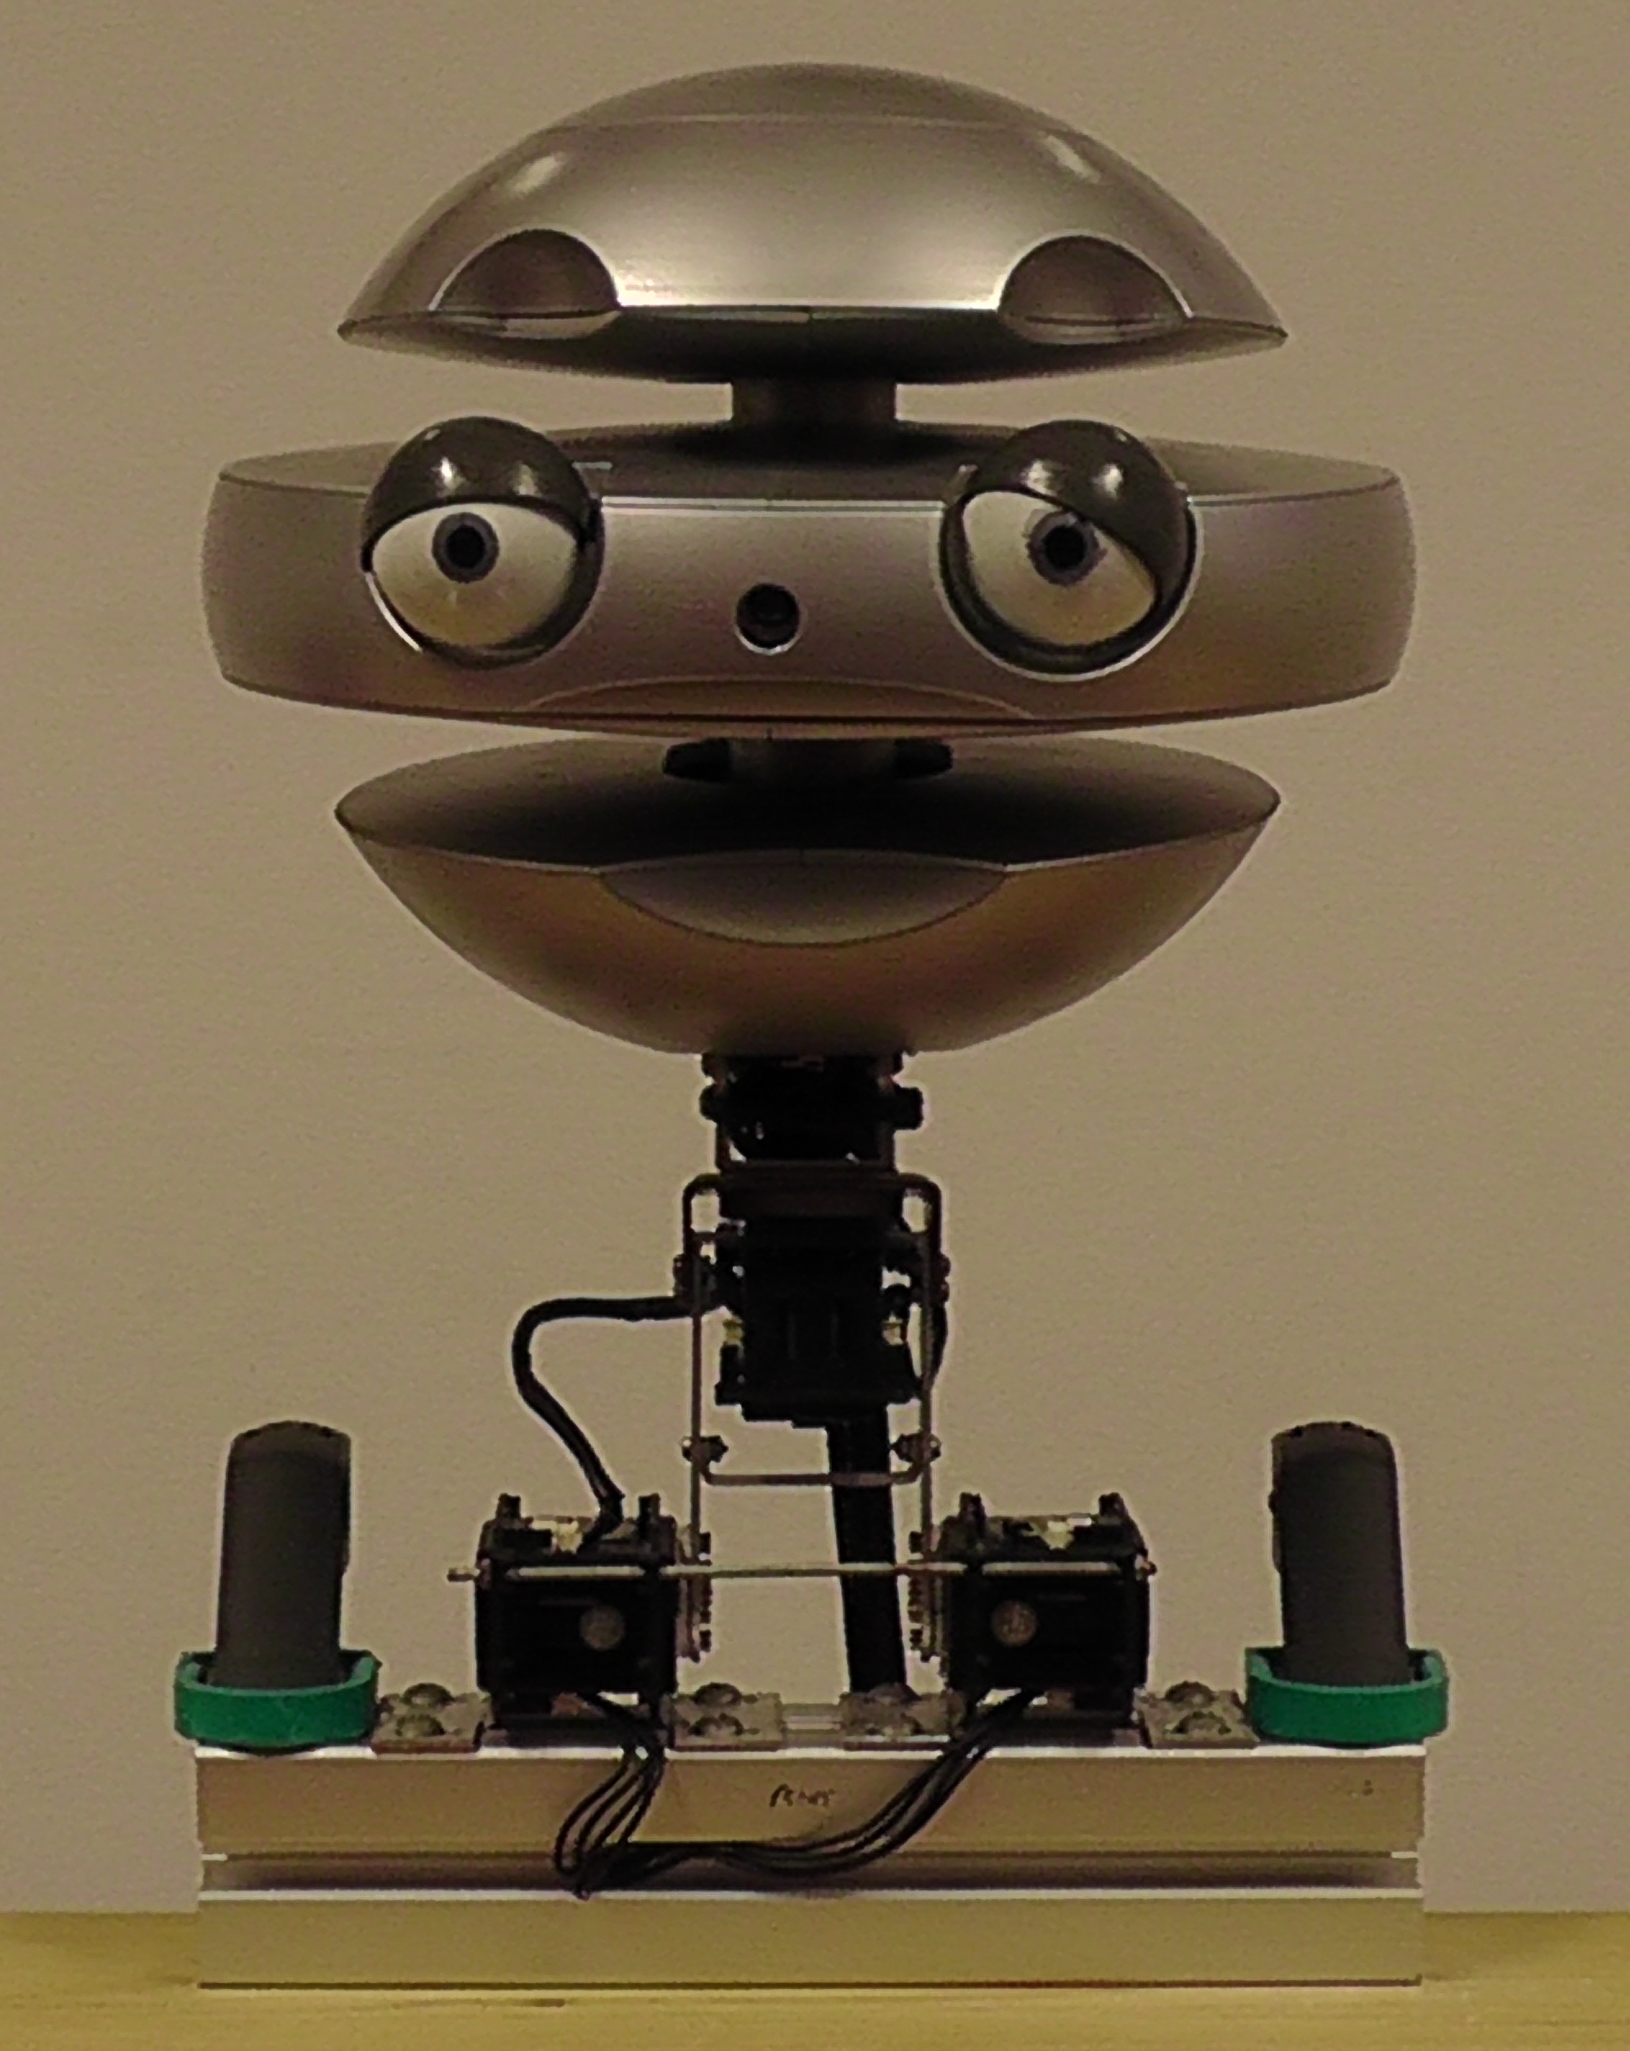
\includegraphics[width=\columnwidth]{images/gbe/joy.jpg}
        \caption{Joy}
    \end{subfigure}
    \begin{subfigure}{0.2\columnwidth}
        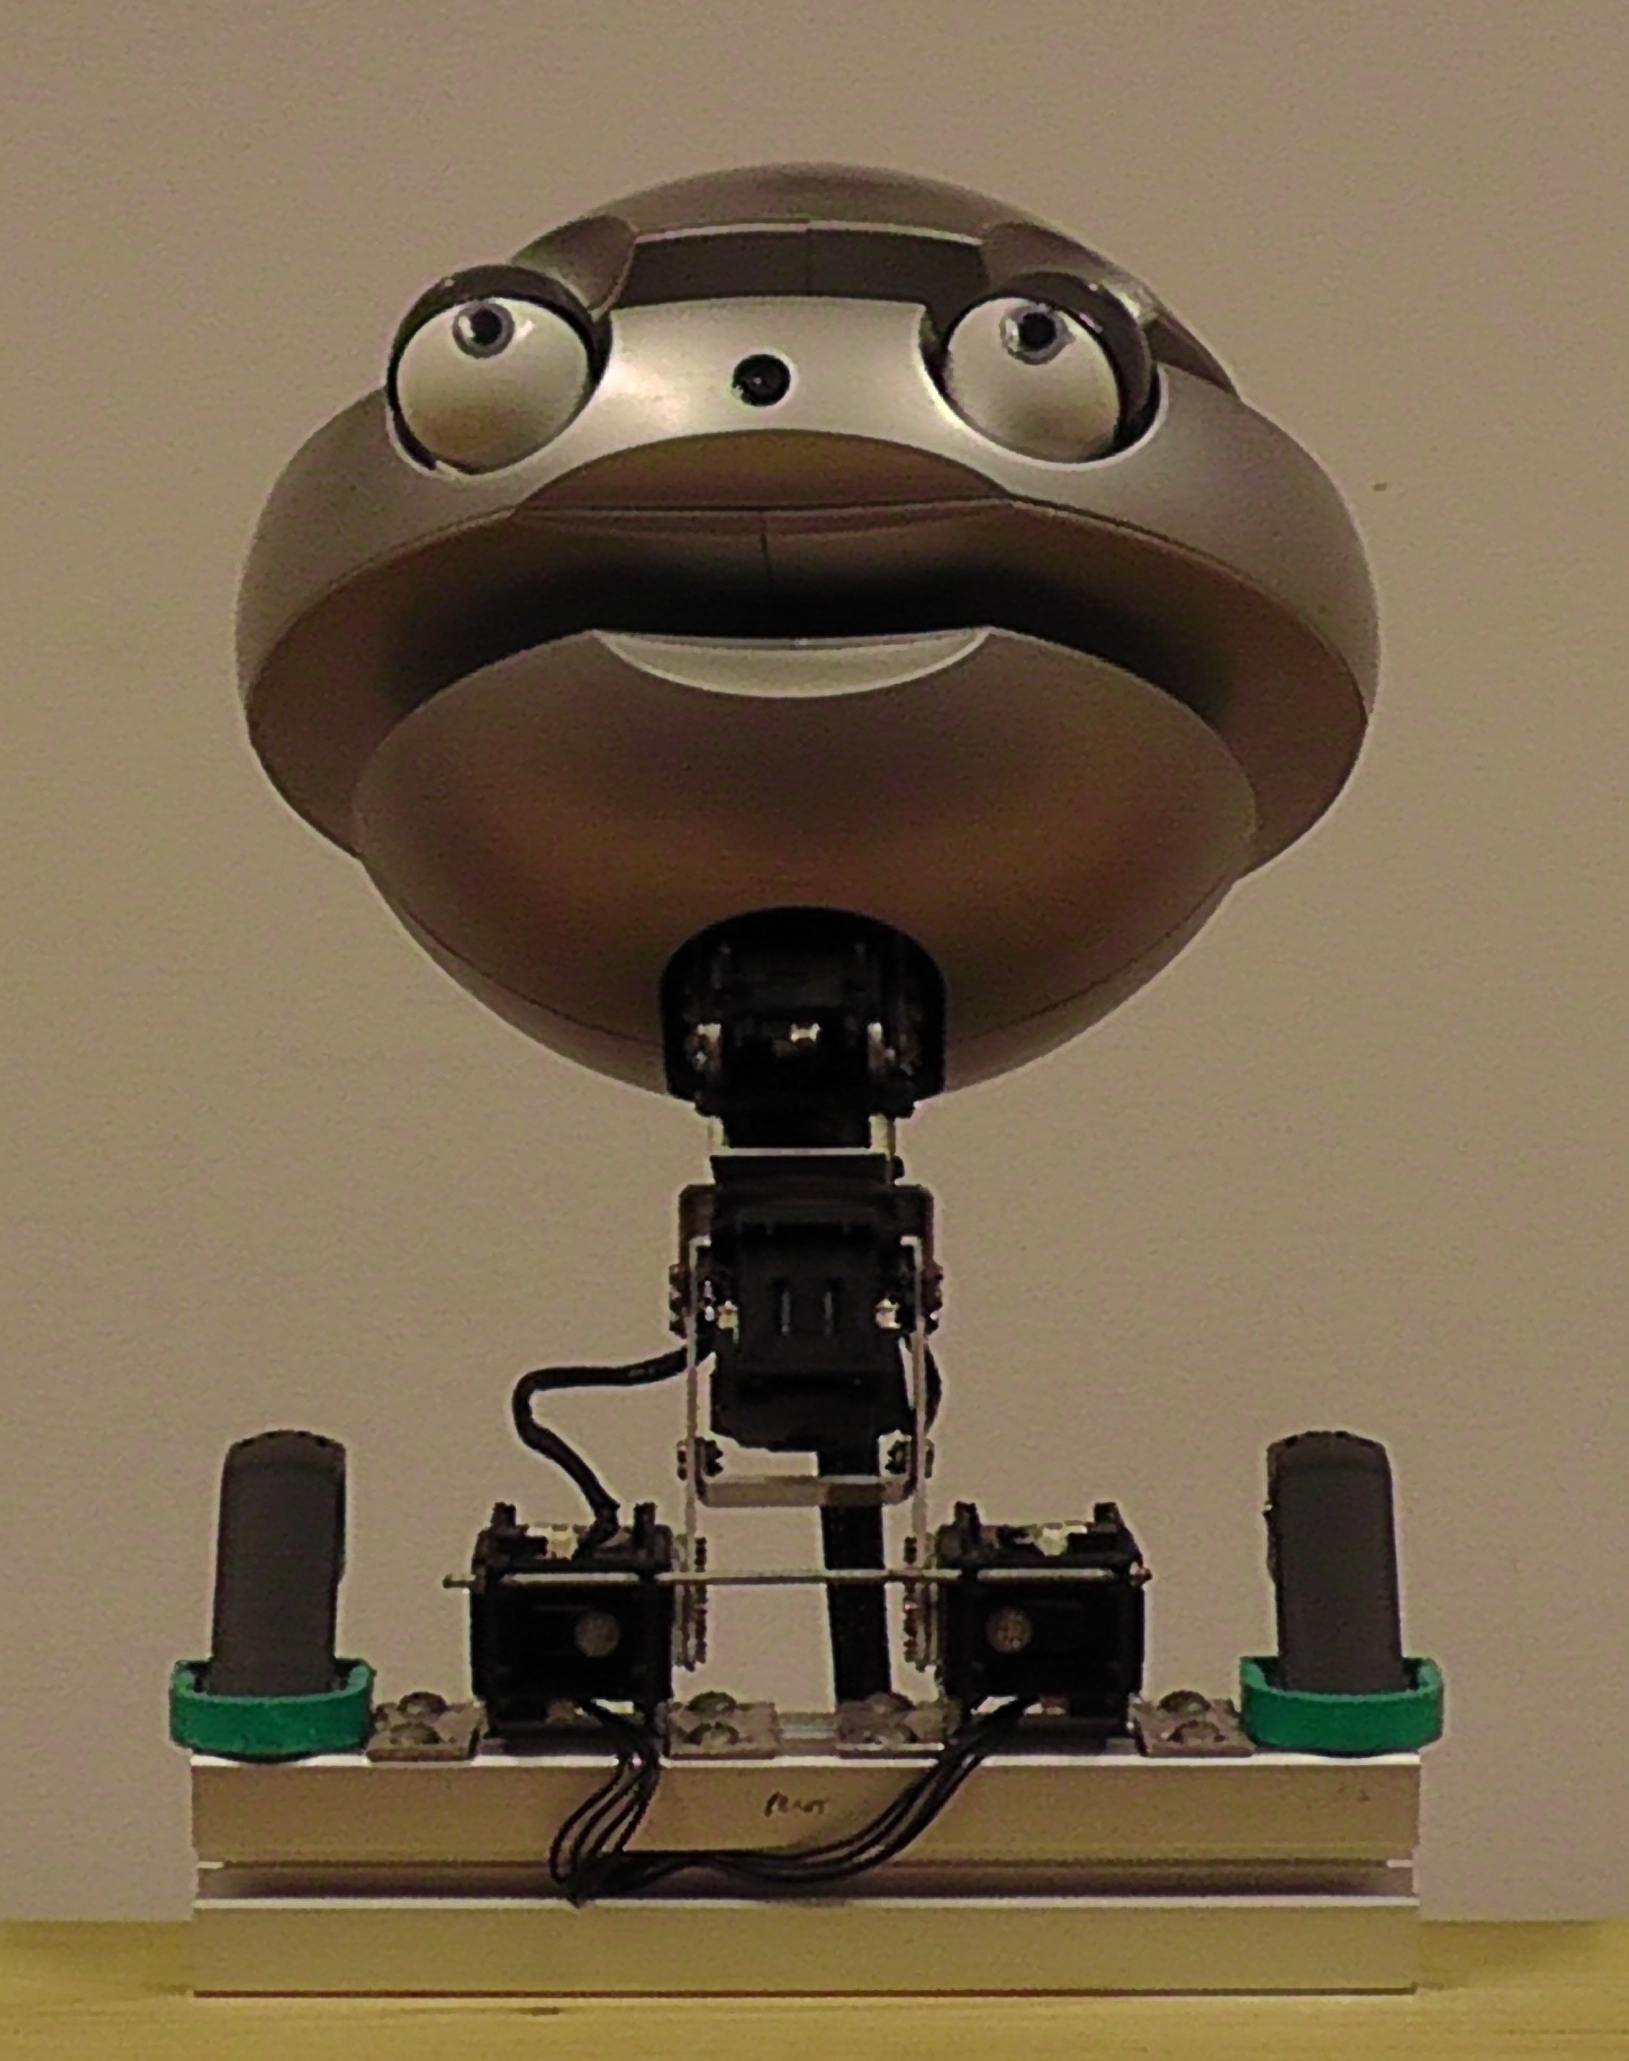
\includegraphics[width=\columnwidth]{images/gbe/pride.jpg}
        \caption{Pride}
    \end{subfigure}
    \begin{subfigure}{0.2\columnwidth}
        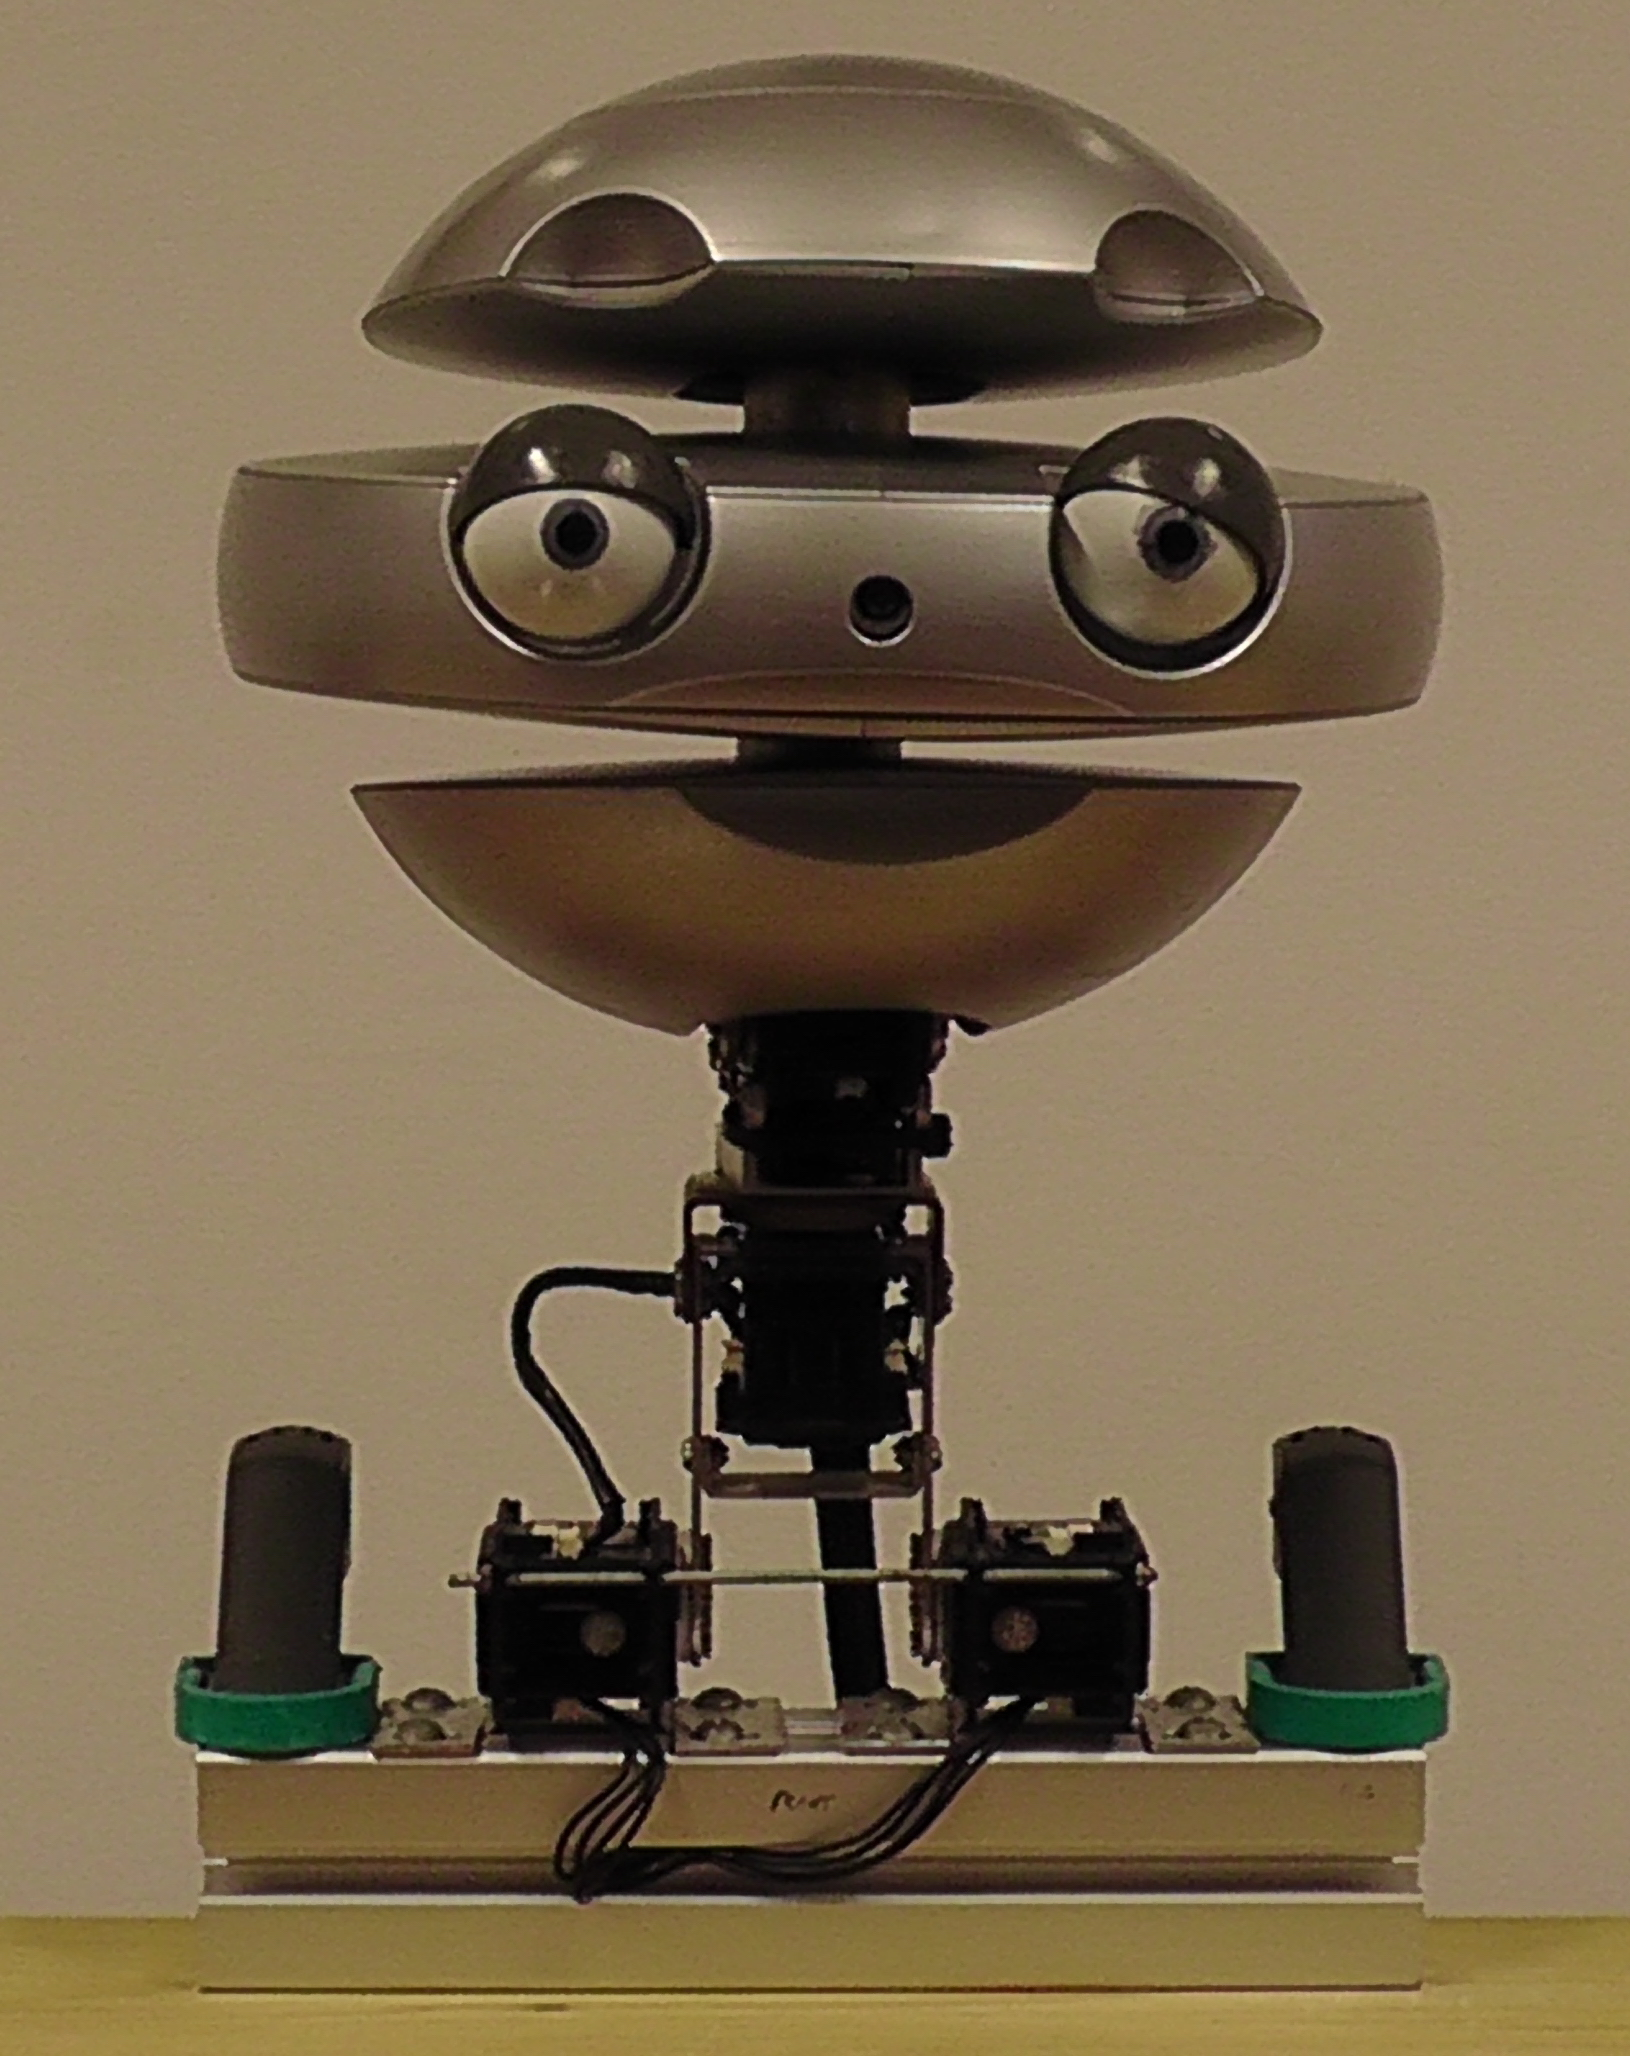
\includegraphics[width=\columnwidth]{images/gbe/admiration.jpg}
        \caption{Admiration}
    \end{subfigure}
    
    \begin{subfigure}{0.2\columnwidth}
        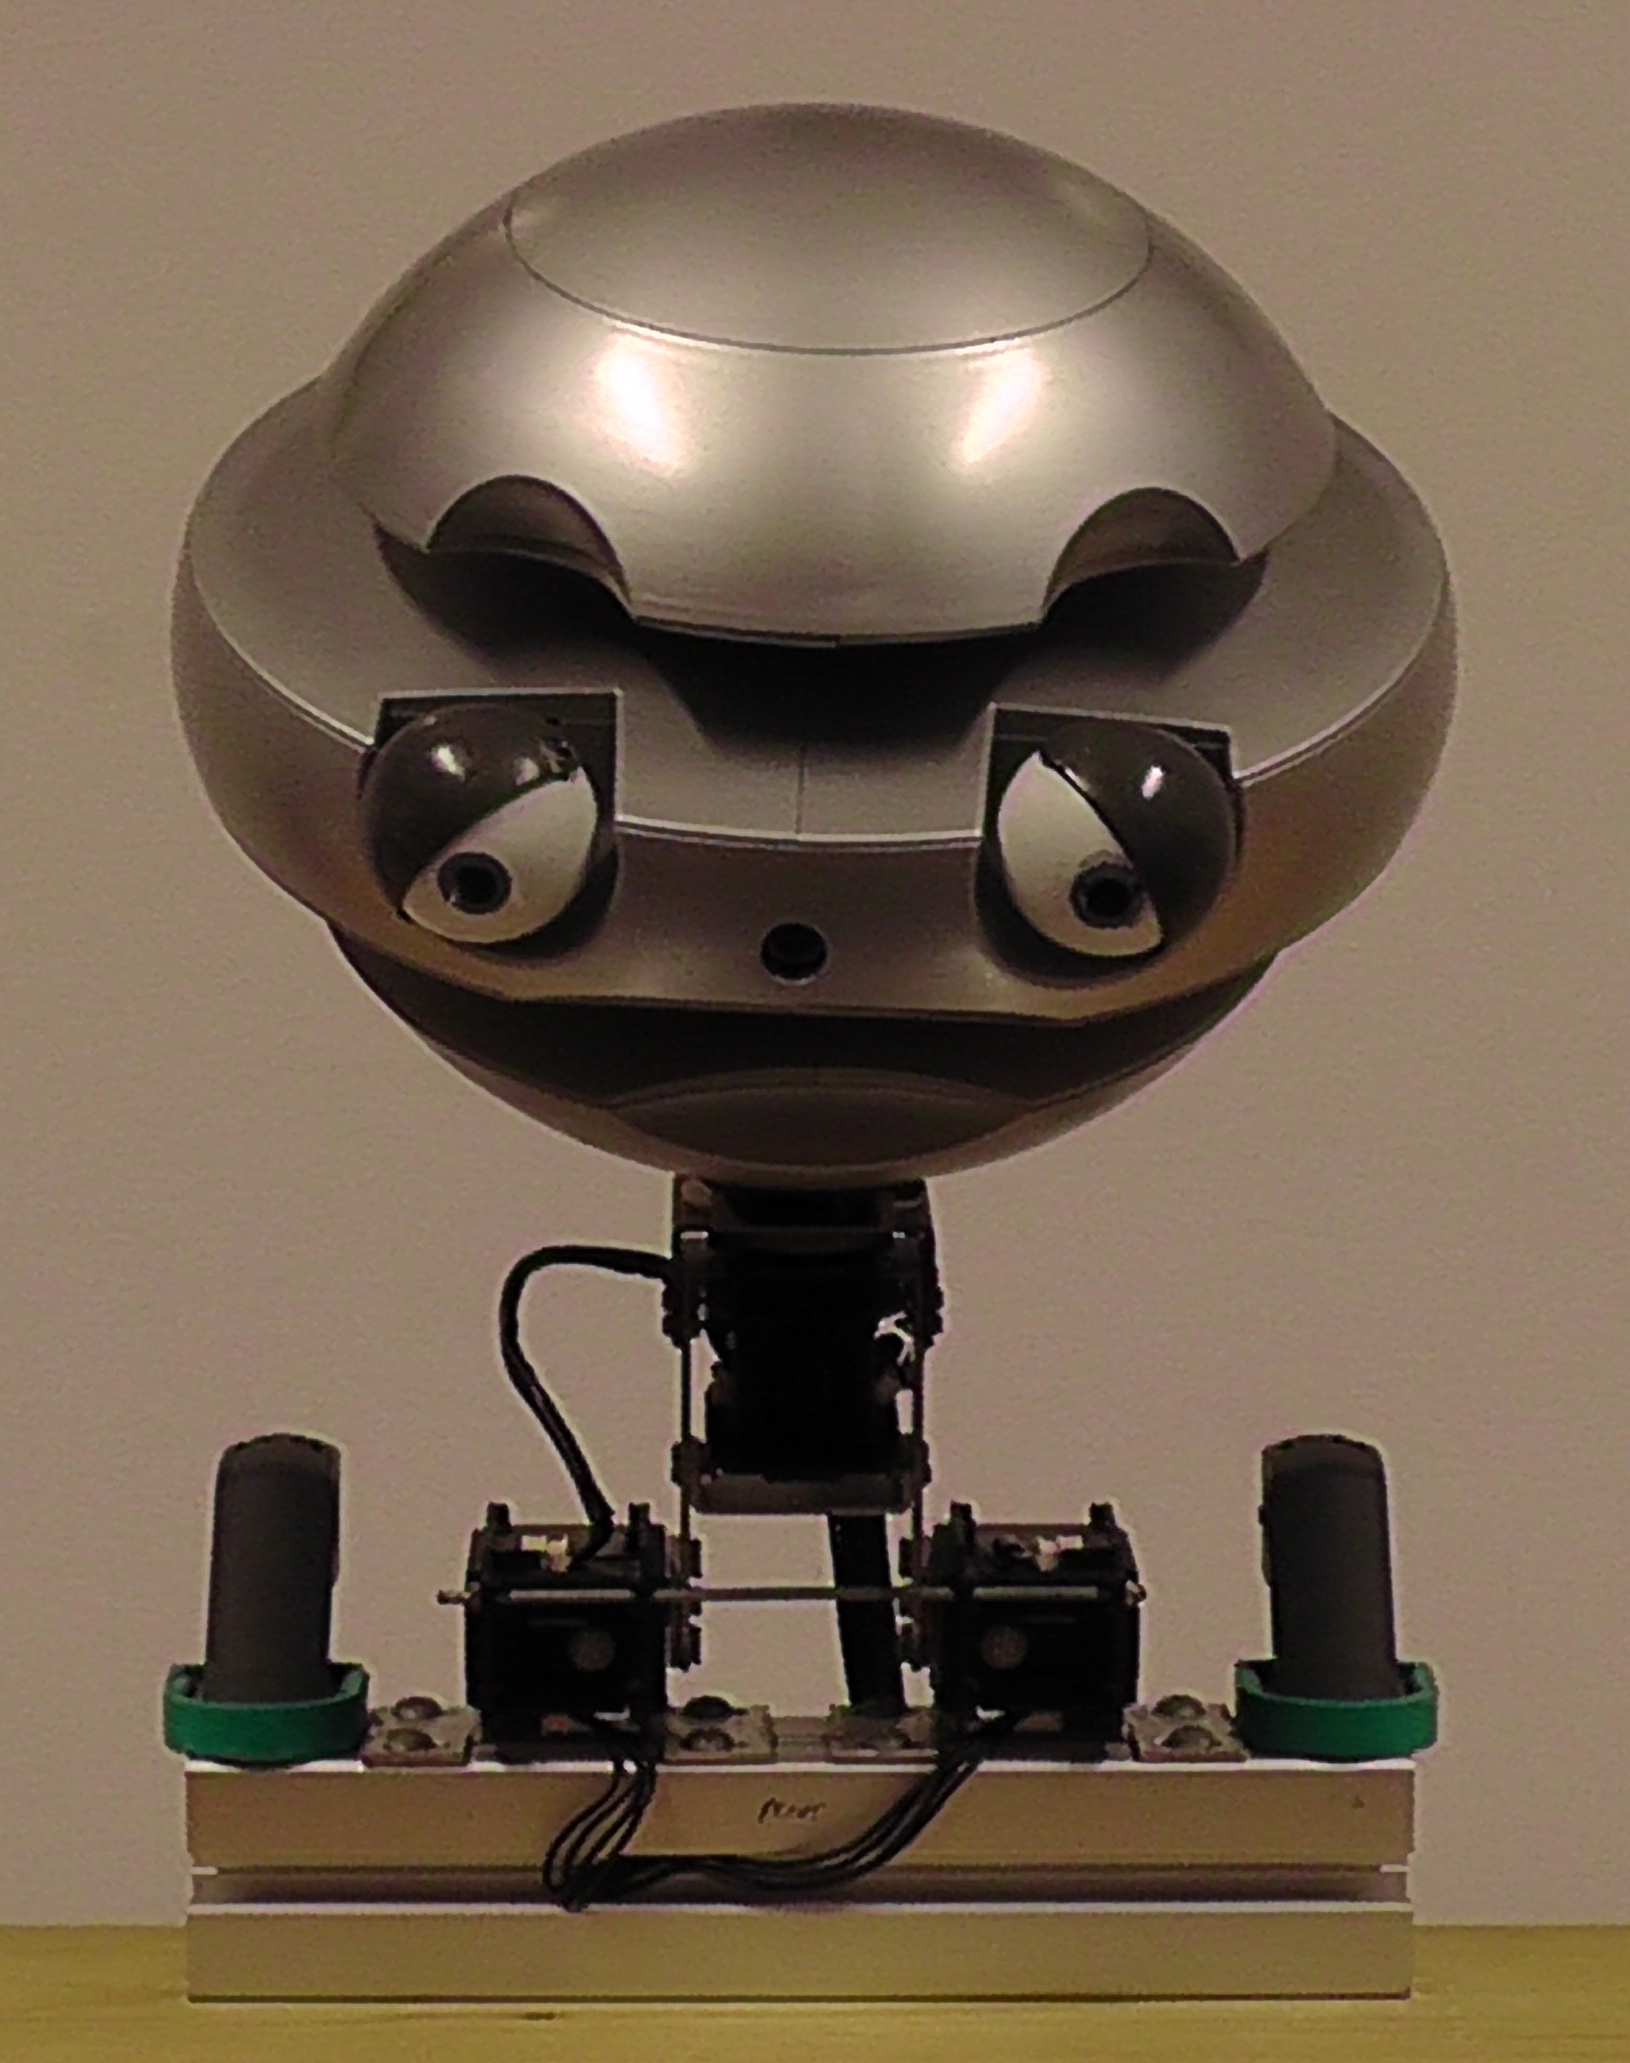
\includegraphics[width=\columnwidth]{images/gbe/distress.jpg}
        \caption{Distress}
    \end{subfigure}
    \begin{subfigure}{0.2\columnwidth}
        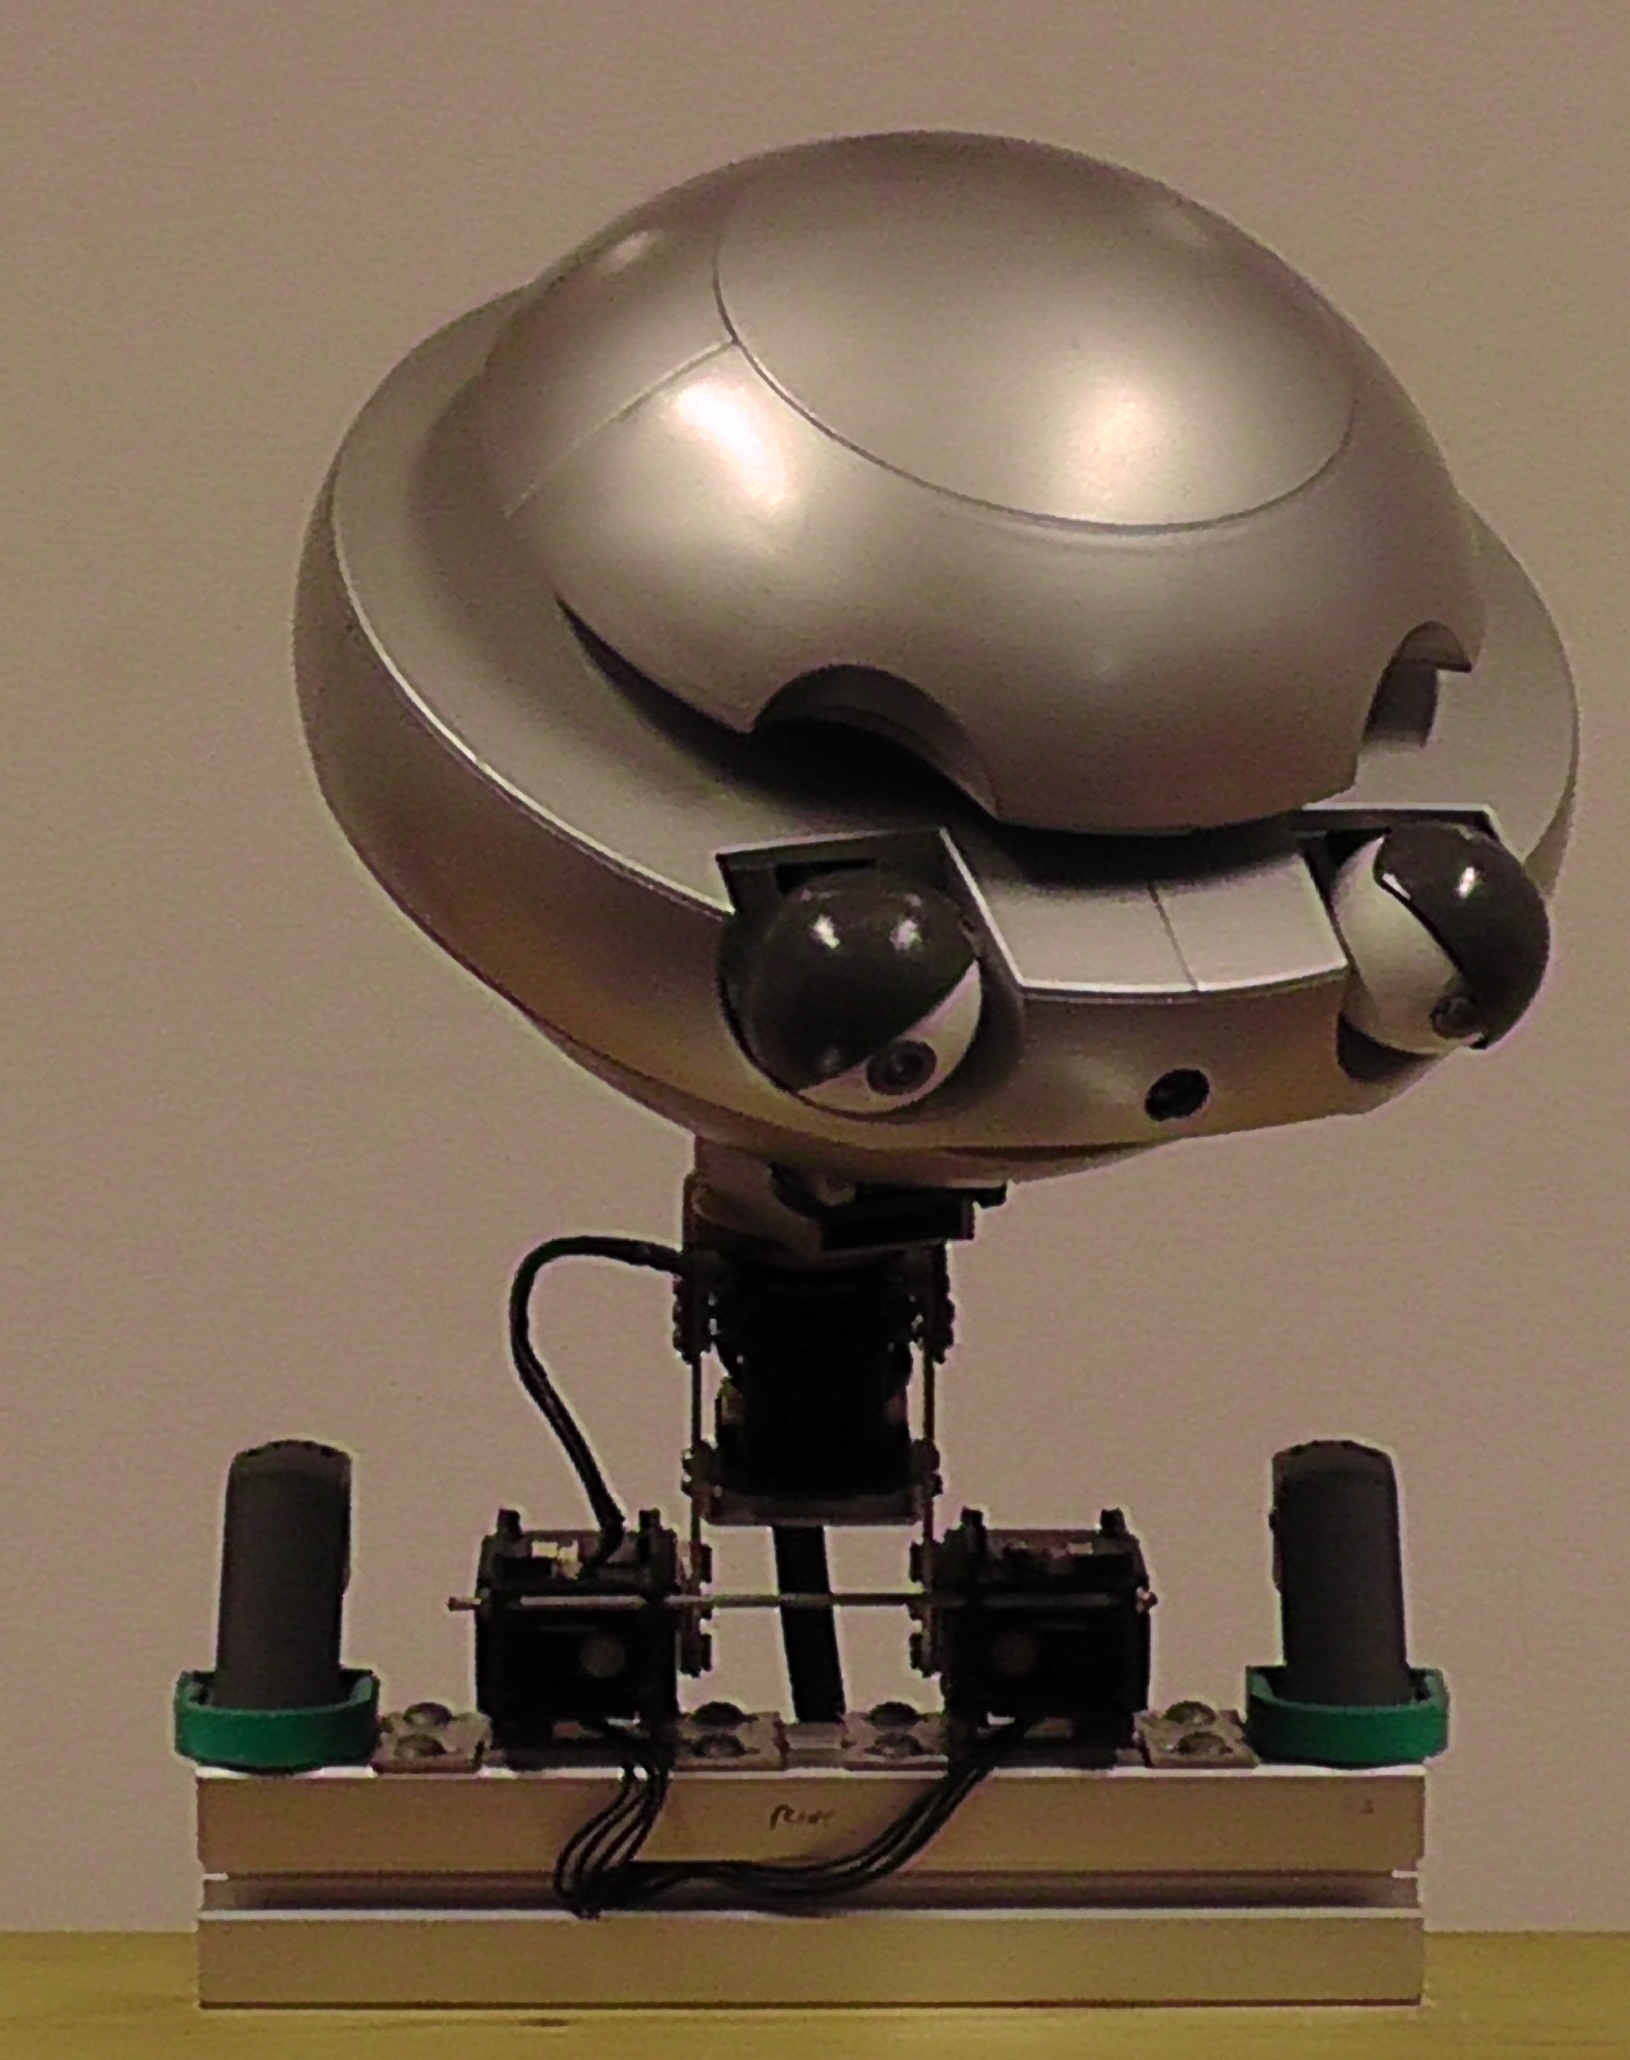
\includegraphics[width=\columnwidth]{images/gbe/shame.jpg}
        \caption{Shame}
    \end{subfigure}
    \begin{subfigure}{0.2\columnwidth}
        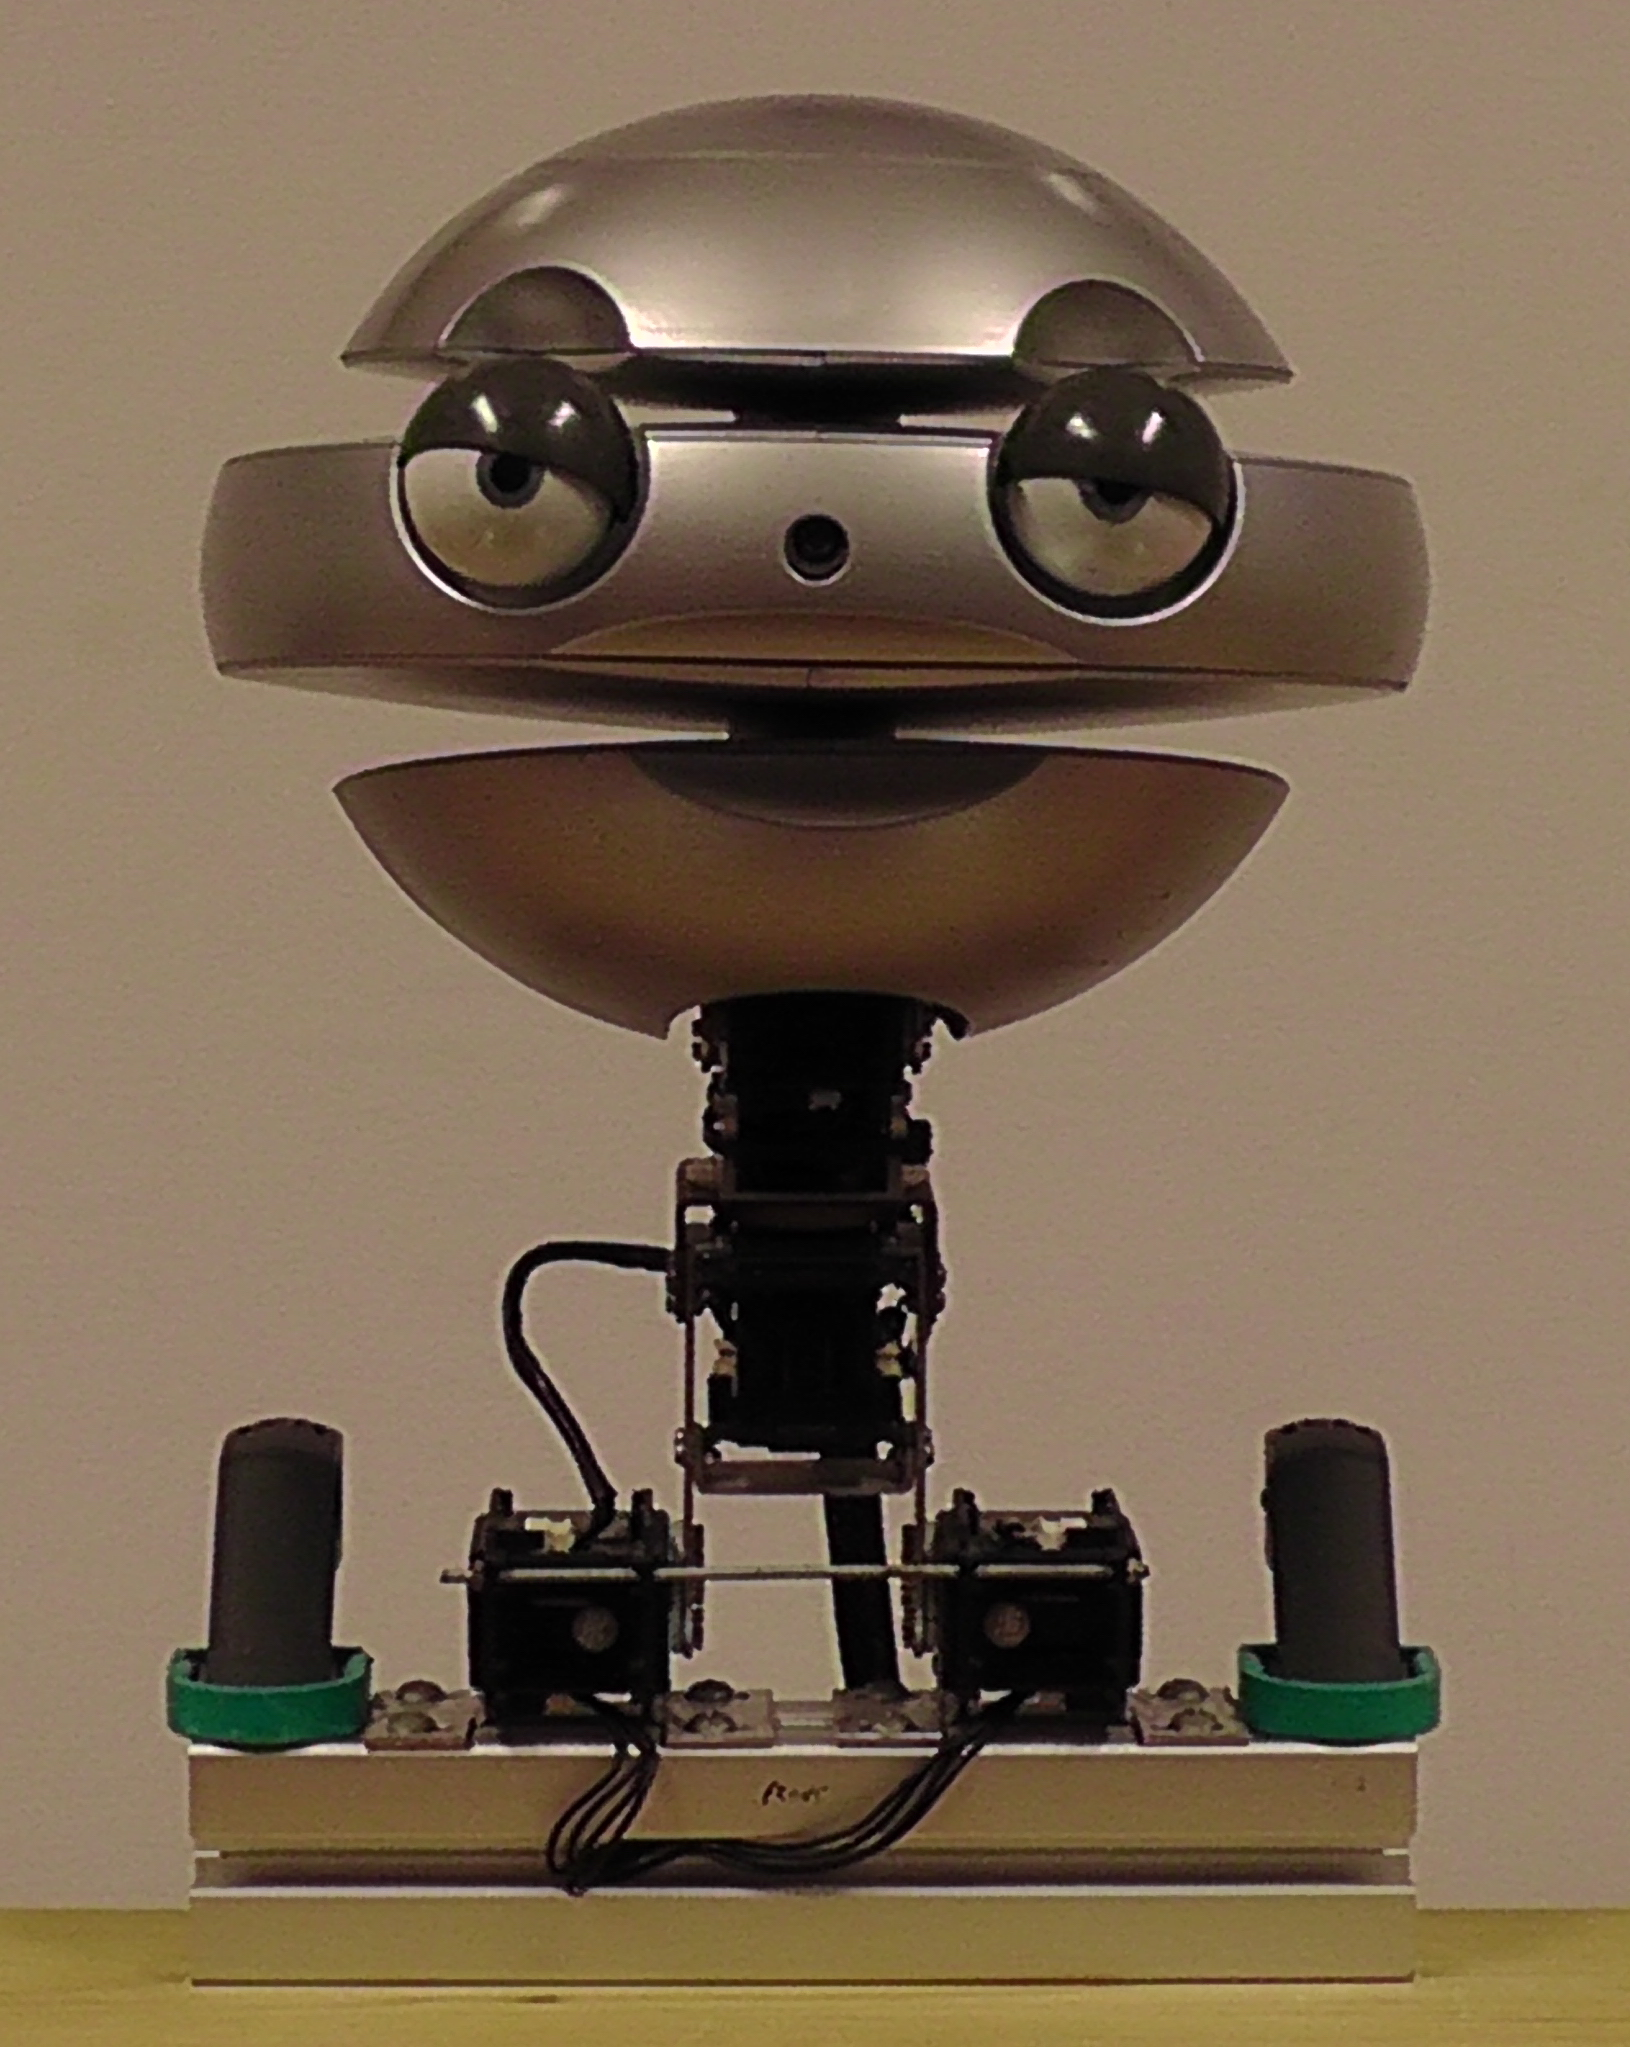
\includegraphics[width=\columnwidth]{images/gbe/reproach.jpg}
        \caption{Reproach}
    \end{subfigure}
    \caption{Postures embodied on the EMYS robot for each emotion.}
    \label{fig:postures}
\end{figure}


\section{User study}
\label{sec:study4}
Using the Sueca scenario described in the previous section, we conducted a user study where two participants form a team with a robot to play the card game. We used the same embodiment -- EMYS robot -- although the robots expressed different types of emotions: group-based or individual-based emotions. Based on the previously discussed findings from intergroup interactions in human-human \cite{kessler2005group,allen2004exploring} as well as in human-robot \cite{kuchenbrandt2013robot,haring2014would,desai2012effects,wang2016trust} scenarios, we expect to check the following hypothesis:

\textbf{H1:} Participants will have a stronger Group Identification with a robotic partner that expresses group-based emotions.

\textbf{H2:} Participants will have a more positive perception of a robotic partner that expresses group-based emotions.

\textbf{H3:} Participants will have a higher degree of Group Trust with a robotic partner that has group-based emotions.


\subsection{Procedure}
Each session of the experiment had two participants and took approximately 45 minutes. Participants read a consent form and were briefly introduced to the game activity. The game rules were described and two researchers played a sample game with the participants over a regular wooden table. Then, participants were randomly assigned to one robotic partner -- which could express either group-based or individual-based emotions--, and moved to the touch table, where they played three consecutive games with the robots, see Figure~\ref{fig:user-study}.
In the beginning one researcher explained how the game works over the touch table and the initial setup of assigning the robots' cards. At the same time, another researcher would set two cameras for video recording if participants had authorised. A researcher stayed in the experiment room until the end of the first trick. After this, both researchers left the room and let participants play the three games. Finally, they were given a questionnaire and the experiment ended with a cinema ticket being randomly awarded to one of the participants.

\begin{figure}[ht]
    \centering
    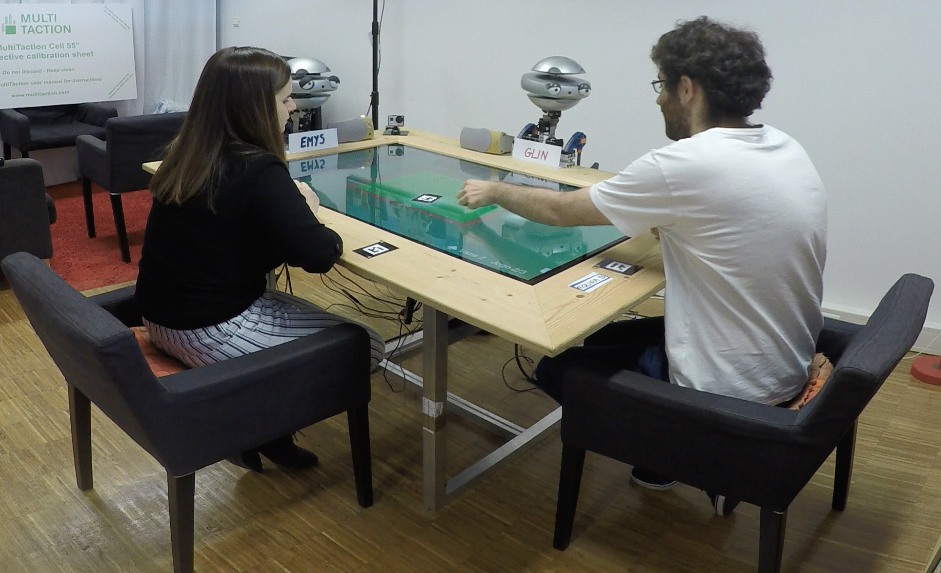
\includegraphics[width=0.7\columnwidth]{images/gbe/interaction}
    \caption{Experimental setting for the user study.}
    \label{fig:user-study}
\end{figure}



\subsection{Measures}
Independently of the robotic partner, all participants answered a  final questionnaire that contained the following measures:
\begin{itemize}
\item \textbf{Group Identification} \cite{leach2008group}
with the Portuguese adaptation \cite{ramos2011adaptaccao} 
to assess the in-Group Identification with their robotic partner;
\item \textbf{Godspeed Questionnaire} \cite{bartneck2009measurement}, using the dimensions of Anthropomorphism, Animacy, Likeability, and Perceived Intelligence regarding their robotic partner;
\item \textbf{Group Trust} \cite{allen2004exploring} to assess the perceived trust by the participants regarding their team in the game;
\item \textbf{Demographic questions}, i.e. gender, age, previous interaction with the EMYS robot, proficiency level in the \textit{Sueca} card game.
\end{itemize}
Both Group Identification and Group Trust measures used 7-points Likert Scales, ranging from Strongly Disagree to Strongly Agree. The Godspeed Questionnaire was assessed in 5-points semantic differential scale.

\subsection{Sample}
We recruited a total of 48 university students (33 males and 15 females) with ages ranging from 19 to 33 years old ($M=25.02\pm 2.98$). 25\% of the participants had already interacted with the EMYS robot and 77.1\% reported at least a medium proficiency level of playing the \textit{Sueca} card game.

\subsection{Results}
In the 24 collected sessions, the team of the robot with group-based emotions won 10 times, lost 11 times, and tied 3 times. Table~\ref{tab:utterances-couning} shows the number of utterances performed by each robot for each emotion and evidences a balanced average of total utterances per session. As expected, in both conditions there were more utterances for positive emotions in general than for negative ones. This can be attributed to the fact that players naturally avoided making bad plays as they were trying to win. Given that some of the following measures did not show normal distributions (as indicated by the Shapiro-Wilk test), we used the non-parametric Mann-Whitney U-test to compare the independent samples.

\begin{table}[ht]
\centering
\caption{Average number of utterances per emotion for the Robot with Group-based Emotions (RGbE) and the Robot with Individual-based Emotions (RIbE).}
\label{tab:utterances-couning}
\begin{tabular}{c|ccccccc|c}
     & Neutral & Admiration & Reproach & Pride & Shame & Joy & Distress & \textbf{TOTAL} \\ \hline
RGbE & 6       & 0          & 0        & 15    & 4     & 4   & 5        & 34             \\
RIbE & 6       & 7          & 2        & 6     & 2     & 4   & 8        & 35            
\end{tabular}
\end{table}



\subsubsection{Group Identification}
A reliability analysis was carried out on the satisfaction and solidarity dimensions comprising 4 and 3 items, respectively. Cronbach's alpha of 0.83 for the satisfaction dimension, and 0.81 for the solidarity dimension indicate a high level of internal consistency for the scale of Group Identification with this specific sample.

We compared the level of Group Identification perceived by the participants towards each robot. Participants had significantly higher levels ($U=175.5, p=0.02, r=0.335$) of Group Identification towards the robotic partner with group-based emotions ($M=5.94\pm0.17$) than towards the robotic partner with individual-based emotions ($M=5.22\pm0.22$), see Figure~\ref{fig:group-measures}.

Additionally, a Spearman's rank-order correlation was run to determine if there was a relationship between the number of points of the team and the Group Identification metric. The rationale was to check if having more points as a consequence of winning the game would also have a positive effect on this dimension. The correlation was non-significant ($r_s=0.153$, $p=0.30$), which suggests that these two factors are independent. 



\begin{figure}[ht]
    \centering
    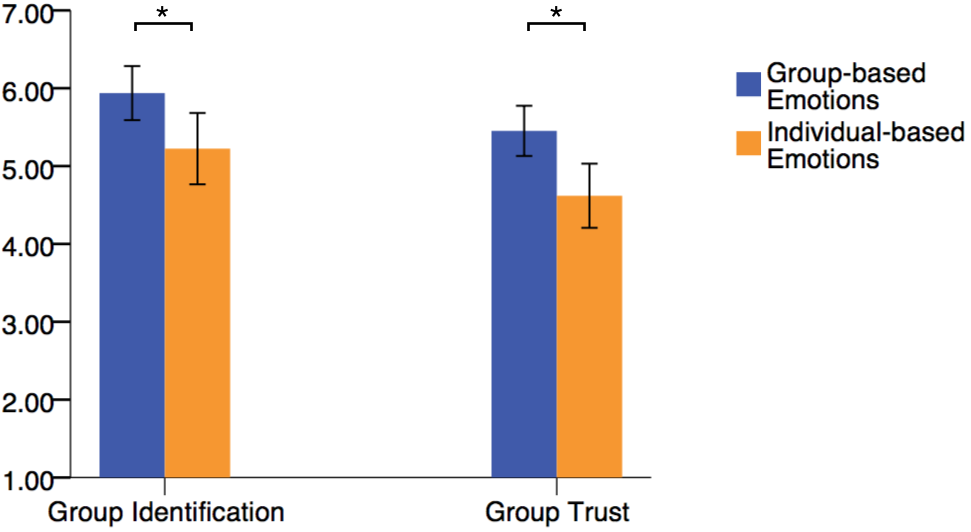
\includegraphics[width=0.6\columnwidth]{images/gbe/group2.png}
    \caption{Group Identification and Group Trust averages attributed to each team with a robot that expresses either group-based or individual-based emotions. (*$p<0.05$)}
    \label{fig:group-measures}
\end{figure}

\subsubsection{Perception of the robots}

To check whether the expression of individual or group-based emotions was influencing the perception of the robots, we compared the levels of Anthropomorphism, Animacy, Likeability and Perceived Intelligence attributed to each robot. Results showed no significant differences in the Anthropomorphism ($U=276, p=0.80$), Animacy ($U=275, p=0.79$), and Perceived Intelligence ($U=200, p=0.07$) levels attributed to robotic partner with group-based emotions ($M_{ant}=2.97\pm0.14;M_{ani}=3.57\pm0.13;M_{pi}=3.91\pm0.14$) and the robotic partner with individual-based emotions ($M_{ant}=2.95\pm0.17;M_{ani}=3.50\pm0.14;M_{pi}=3.47\pm0.17$), see Figure~\ref{fig:godspeed}. However, participants attributed significantly higher scores of Likeability ($U=142.0, p=0.002, r=0.437$) to the robotic partner with group-based emotions ($M=4.33\pm0.11$) than the robotic partner with individual-based emotions ($M=3.49\pm0.21$), see Figure~\ref{fig:godspeed}.


\begin{figure}[ht]
    \centering
    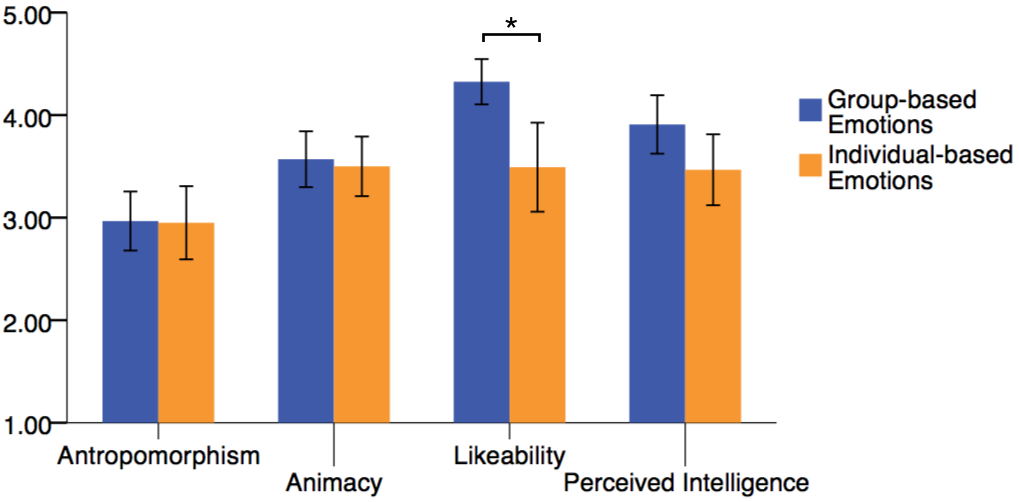
\includegraphics[width=0.7\columnwidth]{images/gbe/godspeed2.png}
    \caption{Averages of Godspeed's dimensions attributed to each robot. (*$p<0.05$)}
    \label{fig:godspeed}
\end{figure}

Additionally, a Spearman's rank-order correlation was run to determine the relationship between Group Identification and the four measured dimensions of the Godspeed Questionnaire. There was a strong, positive, and statistically significant correlations between Group Identification and Anthropomorphism ($r_s=0.529$,  $p<0.01$), Animacy ($r_s=0.318$, $p=0.03$), Likeability ($r_s=0.606$, $p<0.01$), and Perceived Intelligence ($r_s=0.595$, $p<0.01$).

\subsubsection{Group Trust}
A reliability analysis was carried out on the Group Trust scale comprising 7 items, respectively. Cronbach's alpha of 0.74 indicates a high level of internal consistency for this scale with this specific sample.

To check whether the portrayal of individual or group-based emotions was influencing the group trust, we compared the Group Trust levels of each human-robot team. Results showed a statistically significant difference of Group Trust ($U=148, p<0.01, r=0.417$). Partners of the robot with group-based emotions reported significantly higher levels of Group Trust ($M=5.45\pm0.16$) than participants partnering the robot with individual-based emotions ($M=4.62\pm0.20$), see Figure~\ref{fig:group-measures}.

Additionally, a Spearman's rank-order correlation was run to determine the relationship between Group Trust and the number of points of the team. Again, there was no significant correlation between the Group Trust and the number of points ($r_s=0.158$, $p=0.28$).

\section{Discussion}
\label{sec:study4-discussion}
Overall, the following conclusions can be drawn from the obtained results. \textbf{H1} predicted a stronger Group Identification with a robotic partner that expresses group-based emotions. Indeed, the expression of group-based emotions lead to higher levels of Group Identification. This result seem to be coherent with previous findings from the social psychology, where group-based emotions are an antecedent of Group Identification \cite{kessler2005group}.

Our results also partially support \textbf{H2}, which predicted a more positive perception of a robotic partner that expresses group-based emotions. Although participants perceived both robots similarly in terms of Anthropomorphism, Animacy, and Perceived Intelligence, they rated the robotic partner that expresses group-based emotions with significantly higher levels of Likeability. Our expectation was in-line with previous findings \cite{kuchenbrandt2013robot,haring2014would}, where the perceived group identity of a robot had a significant impact on how the robot is perceived. However, their manipulation of group identity referred to the extremes of belonging to the in-group or the out-group, stressing a stronger difference of Group Identification when compared to our setting. Therefore, even with a statistically significant difference of the Group Identification (H1), it was not prominent enough to elicit differences on the Anthropomorphism, Animacy, and Perceived Intelligence. Nevertheless, tendencies can be inferred in both Figure~\ref{fig:godspeed} and in the positive and significant correlations between the level of Group Identification and the measured dimensions of the Godspeed Questionnaire.

According to \textbf{H3}, we expected a higher degree of Group Trust with a robotic partner that has group-based emotions. This was confirmed as participants that were in the team of the robot that expresses group-based emotions attributed a higher level of trust towards the team. We believe this result is relevant for the emerging field of Human-Robot Teams, as trust constitutes one the most important constructs to support effective interaction and cooperation \cite{hancock2011meta}. Furthermore, trust and social identity have been postulated as antecedents of positive team performance \cite{allen2004exploring}.


\section{Concluding Remarks}
\label{sec:conclusind-remarks}
As human-robot groups become more prevalent, it is important to explore new ways of improving their interactions and creating effective collaborations. Therefore, this work provides a first exploration of group-based emotions in social robotic partners and tries to understand their impact on human-robot teams. The contributions are two fold. First, a model for generating group-based emotions on social robots is proposed. This model enabled the development of two distinct robotic characters that express either individual or group-based emotions. Second, it also contributes with a user study, where two fully autonomous robots formed two human-robot teams to play a competitive card game. We compared participants' perceptions, Group Identification, and Group Trust towards their robotic partners. The results show that the expression of group-based emotions by a social robotic partner led participants to rate it as more likeable, to trust it more as a team member and also to identify a stronger social group. Overall, group-based emotions were able to emphasise important aspects of the human-robot collaboration, as trust and group identification, revealing a promising role on the design of social robotic team partners.

One limitation of our study is related with the \textit{Sueca} scenario, as the generation of emotions is strongly related to the game itself. On the one hand, it is a very natural scenario for the interaction of autonomous robots with two people. On the other hand, it may result in an unbalanced number of positive emotions when compared to negative emotions in each game. As future work, it is important to explore scenarios where more negative events also occur. Additionally, the study reported here only analysed mixed human-robot teams of two. In the future, it would be important to analyse the effects of group-based emotions in larger teams as well. Finally, the fact that the robots used different wordings in their utterances could have generated a potential confound. For this reason, it would be interesting to analyse the effect of group-based emotions in a scenario with no use of verbal dialogue.

Our final argument is that social emotions such as shame or pride, which go beyond more basic emotions \cite{ekman1987universals}, should be given more attention in the creation of social robots, particularly in human-robot teams. The work presented here takes a step in this direction as it employs a more rich emotional model enabling social robots to autonomously produce more diverse emotional behaviour.